\documentclass{article}

\usepackage[utf8]{inputenc}
\usepackage{graphicx}
\usepackage[catalan]{babel}
\usepackage{dirtytalk}
\usepackage{titlesec}
\usepackage[hidelinks]{hyperref}
\usepackage[T1]{fontenc}

\setlength{\parindent}{0pt}

%----------------------------------------------------------------------------------------
%	TITLE PAGE
%----------------------------------------------------------------------------------------

\newcommand*{\titleGM}{\begingroup % Create the command for including the title page in the document
\hbox{ % Horizontal box
\hspace*{0.2\textwidth} % Whitespace to the left of the title page
\rule{1pt}{\textheight} % Vertical line
\hspace*{0.05\textwidth} % Whitespace between the vertical line and title page text
\parbox[b]{0.75\textwidth}{ % Paragraph box which restricts text to less than the width of the page

{\noindent\Huge\bfseries AndroShopping \\}\\[2\baselineskip] % Title
{\large \textit{Llenguatges de Programació \\\\ 2014 - 2015}}\\[4\baselineskip] % Tagline or further descriptio


\vspace{0.5\textheight}
\begin{flushright}
Albert Lloveras (ls27332)\\
Manel Roca (ls27599)
\end{flushright}
{\noindent}
\\[\baselineskip] % Publisher and logo
}}
\endgroup}

%----------------------------------------------------------------------------------------
%	BLANK DOCUMENT
%----------------------------------------------------------------------------------------

\begin{document}

\pagestyle{empty} % Removes page numbers

\titleGM % This command includes the title page

\tableofcontents

\newpage
\pagestyle{plain}


\section{Introducció}
Aquest any a l'assignatura de llenguatges de programació ens han encarregat el desenvolupament d'una App per a sistemes Android per gestionar les compres d'una botiga.\\

En quant a requeriments, ens han demanat que l'aplicació sigui capaç de sincronitzar les seves dades amb una base de dades a la qual accedirem a través d'un WebService. Per ser més concisos, l'adreça del WebService que se'ns ha proporcionat és:\\

\begin{center}
\url{http://www.v2msoft.com/curso-android/ws/}
\end{center}

De l'anterior WebService se'ns han proporcionat les següents rutes:
\begin{itemize}
	\item  \textbf{http://www.v2msoft.com/curso-android/ws/last\_update.php}:\\
	Aquesta ruta ens permet conèixer la data de la última modificació de la Base de Dades (en format JSON) per tal de determinar si cal o no descarregar-nos de nou les dades al terminal mòbil.
	\item \textbf{http://www.v2msoft.com/curso-android/ws/lista\_productos.php}:\\
	Aquesta ruta ens retorna un array d'objectes JSON que representen els productes disponibles per la venda al nostre establiment.
\end{itemize}

A l'hora de parlar de funcionalitats de la nostre App, hem de definir primerament que l'aplicació tindrà un seguit d'usuaris els quals podran tenir dos rols:
\begin{itemize}
	\item Rol usuari:\\
	Aquest tipus d'usuari serà el bàsic de la aplicació i només podrà realitzar operacions de modificació del seu perfil, realitzar compres dels productes disponibles a l'establiment i consultar el seu històric de compres realitzades.
	\item Rol admin:\\
	Aquest tipus d'usuari estarà reservat només als responsables de l'establiment. D'aquesta manera, les funcionalitats que presenta són lleugerament diferents a les citades anteriorment. Per ser més concrets, aquest rol d'usuari permetrà manegar els usuaris de la aplicació, manegar els productes de l'establiment i tenir un seguiment de totes les ventes realitzades amb la possibilitat de consultar quin client ha fet cada compra.
\end{itemize}

Finalment, cal destacar que els requeriments tècnics a nivell de Android són que la nostre App ha de ser compatible amb la SDK 15 en amunt i una versió de Android 4.4.0 o superior. No obstant, se'ns ha demanat un disseny i programació optimitzats per a la SDK 22 i versió de Android 5 o superior.


\section{Diagrama de classes}

\begin{center}
	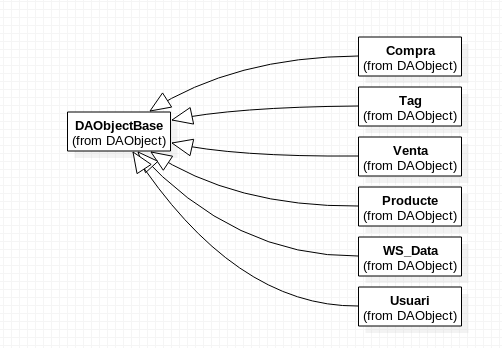
\includegraphics[scale=0.5]{img/1.png}
	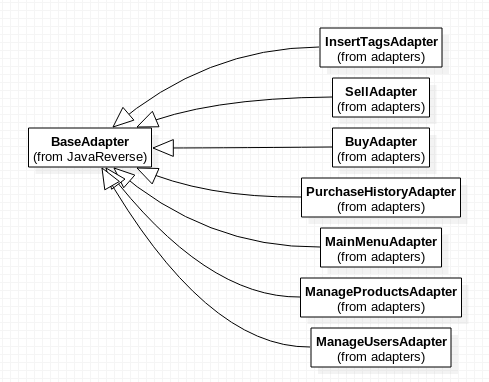
\includegraphics[scale=0.5]{img/2.png}
	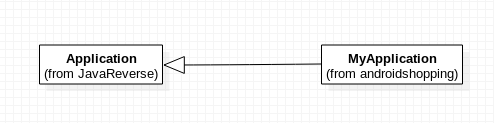
\includegraphics[scale=0.5]{img/3.png}
	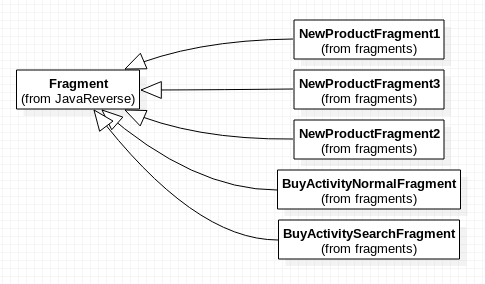
\includegraphics[scale=0.5]{img/4.png}
	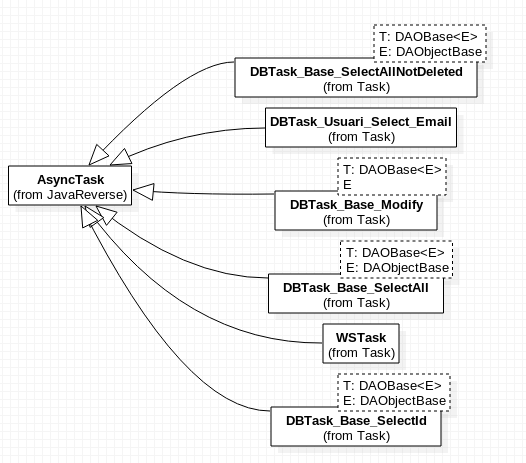
\includegraphics[scale=0.5]{img/5.png}
	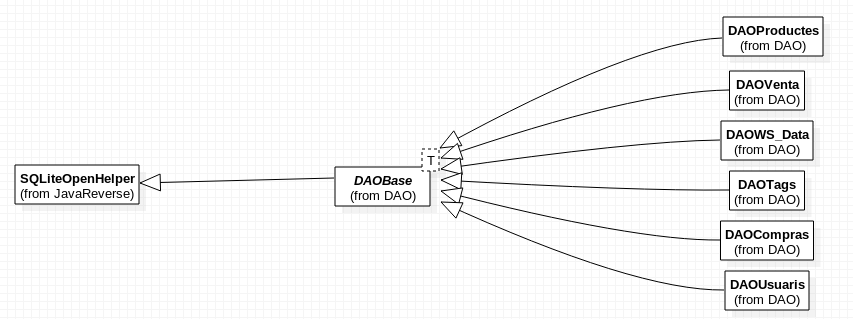
\includegraphics[scale=0.5]{img/6.png}
	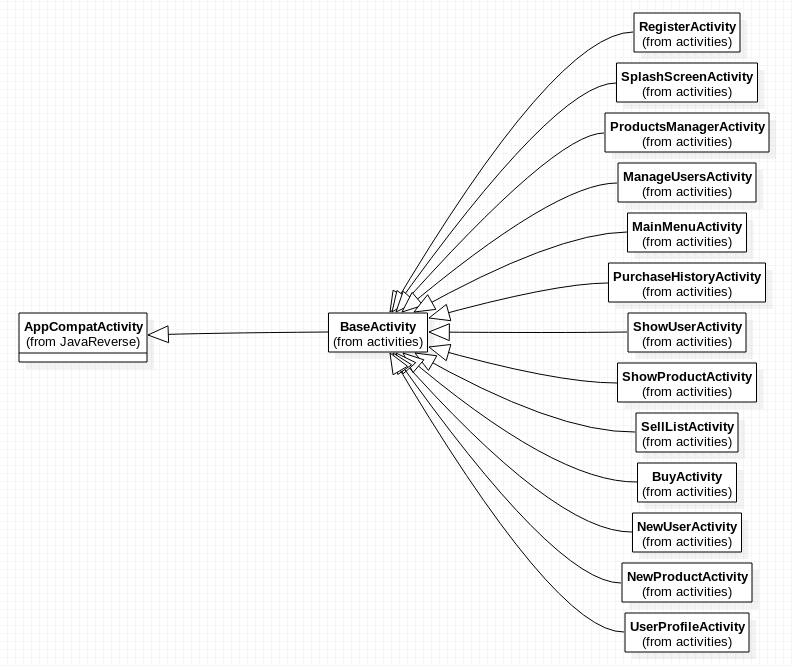
\includegraphics[scale=0.5]{img/7.png}
\end{center}

\newpage
\section{Diagrama BBDD}
\begin{center}
	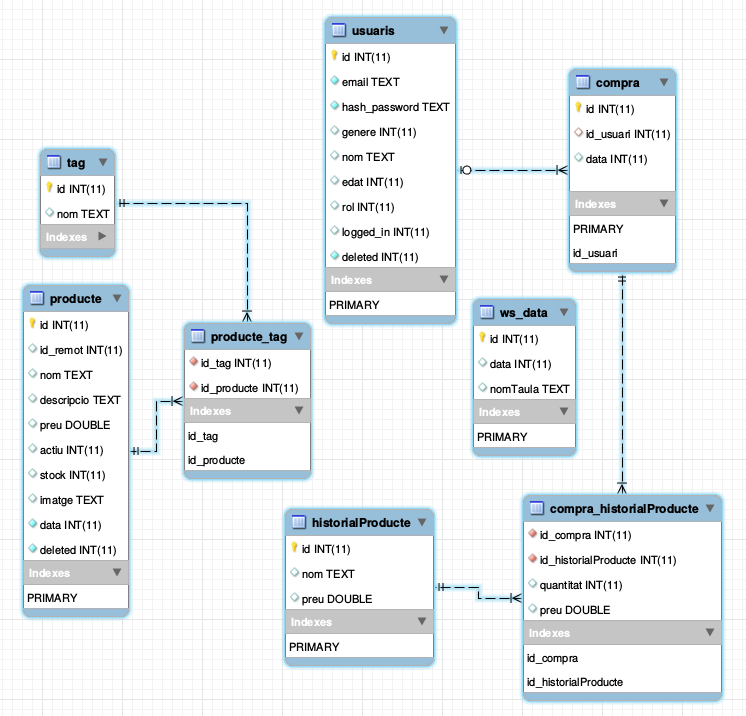
\includegraphics[scale=0.5]{img/Android_DB_Schema.png}
\end{center}

\newpage
\section{Conclusions}
Les conclusions de la realització d'aquesta pràctica de llenguatges de programació són:\\

En primer lloc, posar en pràctica, de forma conjunta, tots els conceptes vistos a classe durant el semestre. Això ha servit per veure la potencia real del contingut explicat així com també detectar possibles problemes a l'hora d'integrar diverses funcionalitats vistes a classe en problemes reals (càrrega d'imatges mitjançant asynctasks -> out of memory error).\\

Per ser més concrets, hem practicat i molt tot el tema de concurrència, threads i bases de dades. Això ens ha ajudat a reflexionar sobre la importància de definir-se una bona estructura de classes (DAOs i altres) per tal de fer que l'accés a la BBDD sigui prou còmode i escalable, ja que no saps mai, en un futur, quins canvis et poden demanar.\\

Per altra banda, hem descobert i aprés a utilitzar Picasso, que ens ha ajudat moltíssim a gestionar l'accés a les imatges que s'havien de mostrar en les pantalles de la nostre aplicació.  A més a més, hem utilitzat la llibreria Jackson per tal de fer-nos més fàcil la interacció amb els valors de retorn del WebService. 

Per si tot això fos poc, a nivell de programació multiprocés i concurrent, hem aprés a sincronitzar diferents threads mitjançant l'ús de listeners i interfícies.

Finalment, destacar que la realització d'aquesta pràctica també ens ha fet acostumar-nos al nou entorn de desenvolupament de Androi (Android Studio), ja que l'any passat vàrem treballar amb Eclipse. A més, dins d'aquests canvis d'IDE ens hem hagut de familiaritzar amb els nous fitxers de configuració de Gradle per tal d'importar les llibreries de manera quasi automàtica.


\end{document}
